\documentclass{article}
\usepackage{graphicx} 
\usepackage{multirow}
\usepackage{enumitem}
\usepackage{amssymb}
\usepackage{amsmath}
\usepackage{xcolor}
\usepackage{cancel}
\usepackage{tcolorbox}
\usepackage{physics}
\usepackage{geometry}
\usepackage{tikz}
\usepackage{tikz-3dplot}
\usepackage{pgfplots, tkz-euclide,calc}
    \usetikzlibrary{patterns,snakes,shapes.arrows,3d}
    \usepgfplotslibrary{fillbetween}
	\geometry{
		total = {160mm, 237mm},
		left = 25mm,
		right = 35mm,
		top = 30mm,
		bottom = 30mm,
	}

\newcommand{\jawab}{\textbf{Solusi}:}
\newcommand{\del}{\partial}
\begin{document}
    \pagenumbering{gobble}
    \begin{tabular}{|lcl|}
     \hline
     Nama&:&Teosofi Hidayah Agung\\
     NRP&:&5002221132\\
     \hline
    \end{tabular}
    \begin{enumerate}
        \item \begin{enumerate}
            \item Perlihatkan bahwa $\vb*{F}(x,y,z)=y^2z^3\vb*{i}+2xyz^3\vb*{j}+3xy^2z^2\vb*{k}$ adalah medan konservatif\\
            \jawab
            \begin{flalign*}
                \curl\vb*{F}&=\begin{vmatrix}
                    \vb*{i}&\vb*{j}&\vb*{k}\\
                    \dfrac{\del}{\del x}&\dfrac{\del}{\del y}&\dfrac{\del}{\del z}\\
                    y^2z^3&2xyz^3&3xy^2z^2
                \end{vmatrix}&\\
                &=\left[6xyz^2-6xyz^2\right]\vb*{i}-\left[3y^2z^2-3y^2z^2\right]\vb*{j}+\left[2yz^3-2yz^3\right]\vb*{k}&\\
                &=0\vb*{i}-0\vb*{j}+0\vb*{k}=0
            \end{flalign*}
            $\therefore\vb*{F}(x,y,z)$ adalah medan konservatif
            \item Carilah fungsi $f(x,y,z)$ sedemikian sehingga $\vb*{F}(x,y,z)=\grad f(x,y,z)$\\
            \jawab
            \begin{flalign*}
                \vb*{F}(x,y,z)&=\grad f(x,y,z)&\\
                y^2z^3\vb*{i}+2xyz^3\vb*{j}+3xy^2z^2\vb*{k}&=\frac{\del f}{\del x}\vb*{i}+\frac{\del f}{\del y}\vb*{j}+\frac{\del f}{\del z}\vb*{k}&\\
                \begin{cases}
                    \dfrac{\del f}{\del x}&=y^2z^3\\\\
                    \dfrac{\del f}{\del y}&=2xyz^3\\\\
                    \dfrac{\del f}{\del z}&=3xy^2z^2
                \end{cases}\implies& \begin{cases}
                    f(x,y,z)&=\displaystyle\int y^2z^3\, dx=xy^2z^3+g(y,z)\\
                    f(x,y,z)&=\displaystyle\int 2xyz^3\, dy=xy^2z^3+h(x,z)\\
                    f(x,y,z)&=\displaystyle\int 3xy^2z^2\, dz =xy^2z^3+l(x,y)
                \end{cases}
            \end{flalign*}
            Ketiga persamaan di atas terpenuhi ketika $g(y,z)=h(x,z)=l(x,y)=C$ dengan $C$ adalah suatu konstanta sembarang.
            
            $\therefore f(x,y,z)=xy^2z^3+C$
        \end{enumerate}
        
        \item Gunakan kebenaran Teorema Green untuk $\vb*{F}(x,y,z)=(x^2+y^2)\vb*{i}+2xy\vb*{j}$ dimana $A$ adalah daerah empat persegi panjang yang dibatasi oleh: $x=\pm a$; $y=0$; $y=b$ (hitung dengan Teorema Green dan secara langsung)\\
        \jawab
        \begin{center}
            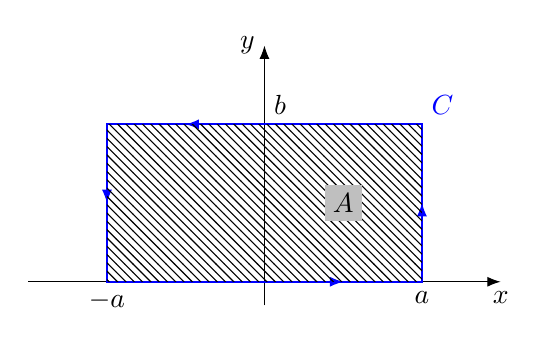
\begin{tikzpicture}
                \draw[-Latex] (-3,0) -- (3,0) node[below] {$x$};
                \draw[-Latex] (0,-0.3) -- (0,3) node[left] {$y$};

                \draw[blue,thick] (-2,0) -- (2,0) -- (2,2) -- (-2,2) -- cycle;
                \draw[blue,smooth,-Latex] (0,0)--(1,0);
                \draw[blue,smooth,-Latex] (2,0)--(2,1);
                \draw[blue,smooth,-Latex] (0,2)--(-1,2);
                \draw[blue,smooth,-Latex] (-2,2)--(-2,1);
                \node[blue] at (2,2) [above right] {$C$};

                \fill[pattern=north west lines] (-2,0) -- (2,0) -- (2,2) -- (-2,2) -- cycle;
                \node at (2,0) [below] {$a$};
                \node at (-2,0) [below] {$-a$};
                \node at (0,2) [above right] {$b$};

                \node at (1,1) [] {\colorbox{lightgray}{$A$}};
            \end{tikzpicture}
        \end{center}
        \begin{itemize}
            \item Dengan Teorema Green
            \begin{flalign*}
                \oint_C \vb*{F}\cdot d\vb*{r}&=\iint_A \left(-\frac{\del}{\del x}(-2xy)-\frac{\del}{\del y}(x^2+y^2)\right)\, dA&\\
                &=\iint_A (-2y-2y)\, dA&\\
                &=-4\int_{-a}^a\int_0^b y\, dy\, dx&\\
                &=-4\int_{-a}^a\left[\frac{1}{2}y^2\right]_0^b\, dx&\\
                &=-2\int_{-a}^a b^2\, dx&\\
                &=-2b^2[a-(-a)]=-4ab^2
            \end{flalign*}
            \item Secara langsung
            \begin{flalign*}
                \oint_C \vb*{F}\cdot d\vb*{r}&=\oint_C (x^2+y^2)\, dx-2xy\, dy&\\
                &=\int_{-a}^a (x^2+0)\, dx-2x(0)d(0) +\int_0^b (a^2+y^2)\, d(a)-2aydy&\\
                &+\int_{-a}^a ((-x)^2+b^2)\, d(-x)-2xb\,d(b)+\int_0^b (0+(-y)^2)\, d(-a)-2(-a)(-y)dy&\\
                &=\cancel{\int_{-a}^a x^2\, dx}-\int_0^b 2ay\, dy-\cancel{\int_{-a}^a x^2\, dx}-\int_{-a}^a b^2\, dx-\int_0^b 2ay\, dy&\\
                &=-4a\int_0^b y\, dx-[b^2x]^a_{-a}&\\
                &=-2ab^2-2ab^2=-4ab^2
            \end{flalign*}
        \end{itemize}
        
        \item untuk menghitung $\displaystyle\oint_C \vb*{F}\cdot d\vb*{r}$ dengan $\vb*{F}=2z\vb*{i}+x\vb*{j}+3y\vb*{k}$ dan $C$ adalah batas luasan elips bidang $z=x$ yang berada dalam silinder $x^2+y^2=4$  yang berorientasi searah dengan putaran jarum jam seperti yang digambarkan jika dilihat dari atas\\
        \jawab\\
        Ilustrasi gambar sebagai berikut
        \begin{center}
            \tdplotsetmaincoords{70}{290}
	\begin{tikzpicture}[tdplot_main_coords,scale=0.65]
		\tikzmath{function a(\x,\y) {return (\x);};}
		\pgfmathsetmacro{\final}{2.0*pi}
		\pgfmathsetmacro{\ejez}{a(-5,0)}
		% The region of integration: the circle of radius 2
		\draw[thick,fill=yellow,opacity=0.5] plot[domain=0:6.2832,smooth,variable=\t] ({2.0*cos(\t r)},{2.0*sin(\t r)},{2.0*cos(\t r)});
		%%% Coordinate axis
		\draw[thick,->] (0,0,0) -- (3.5,0,0) node [right] {\footnotesize$x$};
		\draw[dashed] (0,0,0) -- (-3,0,0);
		\draw[thick,->] (0,0,0) -- (0,3.5,0) node [left] {\footnotesize$y$};
		\draw[dashed] (0,0,0) -- (0,-3,0);
		\draw[thick] (0,0,0) -- (0,0,\ejez);% node [above] {\footnotesize$z$};	
		% The plane: z = x
		\pgfmathsetmacro{\Az}{a(3,3)}
		\pgfmathsetmacro{\Bz}{a(-3,3)}
		\pgfmathsetmacro{\Cz}{a(-3,-3)}
		\pgfmathsetmacro{\Dz}{a(3,-3)}
		\coordinate (A) at (3,3,\Az);
		\coordinate (B) at (-3,3,\Bz);
		\coordinate (C) at (-3,-3,\Cz);
		\coordinate (D) at (3,-3,\Dz);
		% The cylinder
		\foreach \angulo in {0,0.01,...,\final}{
			\pgfmathparse{2.0*cos(\angulo r)}
			\pgfmathsetmacro{\px}{\pgfmathresult}
			\pgfmathparse{2.0*sin(\angulo r)}
			\pgfmathsetmacro{\py}{\pgfmathresult}
			\draw[cyan,opacity=0.1] (\px,\py,-3) -- (\px,\py,3);
		}
		% The intersection of the cylinder and the plane (the trace)
		\draw[blue,thick] plot[domain=0:6.2832,smooth,variable=\t] ({2.0*cos(\t r)},{2.0*sin(\t r)},{2.0*cos(\t r)});
		% Circumference & Ellipse bounding the solid.
		\draw[blue,thick,opacity=0.5] plot[domain=0:6.2831853,smooth,variable=\t] ({2.0*cos(\t r)},{2.0*sin(\t r)},{2.0*cos(\t r)}); 
		%\draw[blue,thick,opacity=0.5] plot[domain=0:6.2831853,smooth,variable=\t] ({2.0*cos(\t r)},{2.0*sin(\t r)},{0.0}); 
		% The plane
		\draw[white] (C) -- (D) node[red,below,sloped,midway]{\footnotesize$x + y + z = 4$};
		\draw[red,dash dot] (A) -- (B) -- (C)	 -- (D) -- (A);
		\fill[pattern color=pink,pattern=north east lines] (A) -- (B) -- (C)	 -- (D) -- (A);
        % The equation of the cyrcumference
		\node[blue,above,sloped] at (0,3,3.5){\footnotesize$x^2 + y^2 = 4$};
		%\fill[pink,opacity=0.5] plot[domain=0:6.2832,smooth,variable=\t] ({2.0*cos(\t r)},{2.0*sin(\t r)},{4.0-2.0*sin(\t r) - 2.0*cos(\t r)});
		% z axis (last part)
		\draw[thick,->] (0,0,\ejez) -- (0,0,5) node [above] {\footnotesize$z$};	
	\end{tikzpicture}
        \end{center}
        Pertama-tama kita perlu mencari vektor normal dari permukaan elips bidang $z=x$. Didapat $\vb*{n}=\dfrac{\vb*{i}-\vb*{k}}{\norm*{\vb*{i}-\vb*{k}}}=\dfrac{1}{\sqrt{2}}(\vb*{i}-\vb*{k})$. Sehingga dengan Teorema Stokes kita dapatkan
        \begin{flalign*}
            \oint_C \vb*{F}\cdot d\vb*{r}&=\iint_S (\curl\vb*{F})\cdot n\,\, d\vb*{S}&\\
            &=\iint_S \begin{vmatrix}
                \vb*{i}&\vb*{j}&\vb*{k}\\
                \del_x&\del_y&\del_z\\
                2z&x&3y
            \end{vmatrix}\cdot \dfrac{1}{\sqrt{2}}(\vb*{i}-\vb*{k})\,\, dS&\\
            &=\dfrac{1}{\sqrt{2}}\iint_S [(3-0)\vb*{i}-(0-2)\vb*{j}+(1-0)\vb*{k}]\cdot (\vb*{i}-\vb*{k})\,\, dS&\\
            &=\dfrac{1}{\sqrt{2}}\iint_S (3\vb*{i}+2\vb*{j}+\vb*{k})\cdot (\vb*{i}-\vb*{k})\, dS&\\
            &=\dfrac{1}{\sqrt{2}}\iint_S (3-1)\, dS&\\
            &=\sqrt{2}\iint_S dS
        \end{flalign*}
        $\displaystyle\iint_S dS$ adalah luas permukaan elips bidang. Dengan rumus luas elips $A=\pi ab$ dengan $a$ dan $b$ masing-masing adalah sumbu minor dan sumbu mayor elips.
        Pada gambar sebelumnya dapat dilihat bahwa sumbu minor $a=2$ dan untuk sumbu mayor dapat dihitung menggunkan Teorema Pythagoras yaitu $b=\sqrt{2^2+2^2}=2\sqrt{2}$. Sehingga 
        \[\iint_S dS=\pi(2)(2\sqrt{2})=4\pi\sqrt{2}\]
        $\therefore\boxed{\displaystyle\oint_C \vb*{F}\cdot d\vb*{r}=\sqrt{2}(4\pi\sqrt{2})=8\pi}$ 
        \item Diketahui medan vektor $\vb*{F}(x,y,z)=27\vb*{i}+x\vb*{j}+z^2\vb*{k}$. Dengan Teorema Gauss, hitung $\displaystyle\iint_S \vb*{F}\cdot d\vb*{S}$ dengan $S$ adalah permukaan benda padat berupa shell silinder (lihat gambar), $1\leq x^2+y^2\leq 16$, $0\leq z\leq 2$.
        \begin{center}
            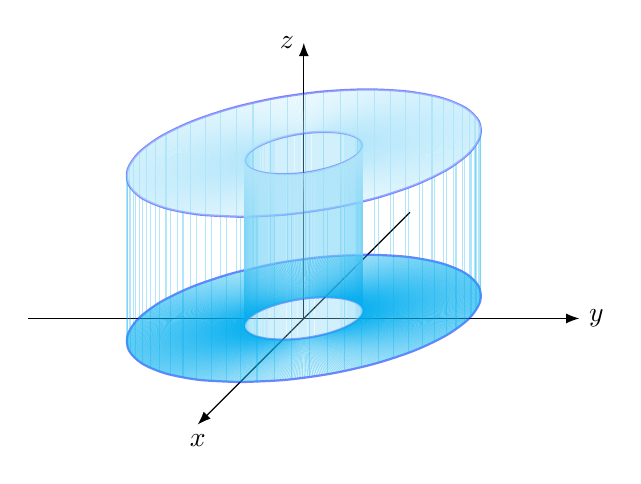
\begin{tikzpicture}[rotate around x=-90,rotate around y=0,rotate around z=-90,scale=0.7]
                \pgfmathsetmacro{\final}{2.0*pi}
                \draw[-Latex] (-5,0,0) -- (5,0,0) node[below] {$x$};
                \draw[-Latex] (0,-5,0) -- (0,5,0) node[right] {$y$};
                \draw[-Latex] (0,0,0) -- (0,0,5) node[left] {$z$};

                \draw[blue,thick,opacity=0.5] plot[domain=0:360,smooth,variable=\t] ({3*cos(\t)},{3*sin(\t)},{3});
                \draw[blue,thick,opacity=0.5] plot[domain=0:360,smooth,variable=\t] ({3*cos(\t)},{3*sin(\t)},{0});

                \draw[blue,thick,opacity=0.5] plot[domain=0:360,smooth,variable=\t] ({1*cos(\t)},{1*sin(\t)},{3});
                \draw[blue,thick,opacity=0.5] plot[domain=0:360,smooth,variable=\t] ({1*cos(\t)},{1*sin(\t)},{0});

                % Big cylinder 
		        \foreach \angulo in {0,0.1,...,\final}{
		        	\pgfmathparse{3*cos(\angulo r)}
		        	\pgfmathsetmacro{\px}{\pgfmathresult}
		        	\pgfmathparse{3*sin(\angulo r)}
		        	\pgfmathsetmacro{\py}{\pgfmathresult}
		        	\draw[cyan,opacity=0.3] (\px,\py,0) -- (\px,\py,3);
		        }
                % Small cylinder
                \foreach \angulo in {0,0.01,...,\final}{
		        	\pgfmathparse{1*cos(\angulo r)}
		        	\pgfmathsetmacro{\px}{\pgfmathresult}
		        	\pgfmathparse{1*sin(\angulo r)}
		        	\pgfmathsetmacro{\py}{\pgfmathresult}
		        	\draw[cyan!50!white,opacity=0.2] (\px,\py,0) -- (\px,\py,3);
		        }
                % roof
                \foreach \angulo in {0,0.01,...,\final}{
		        	\pgfmathparse{1*cos(\angulo r)}
		        	\pgfmathsetmacro{\px}{\pgfmathresult}
		        	\pgfmathparse{1*sin(\angulo r)}
		        	\pgfmathsetmacro{\py}{\pgfmathresult}
		        	\draw[cyan!30!white,opacity=0.4] ({3*\px},{3*\py},3) -- (\px,\py,3);
		        }
                % bottom
                \foreach \angulo in {0,0.01,...,\final}{
		        	\pgfmathparse{1*cos(\angulo r)}
		        	\pgfmathsetmacro{\px}{\pgfmathresult}
		        	\pgfmathparse{1*sin(\angulo r)}
		        	\pgfmathsetmacro{\py}{\pgfmathresult}
		        	\draw[cyan,opacity=0.4] ({3*\px},{3*\py},0) -- (\px,\py,0);
		        }
            \end{tikzpicture}
        \end{center}
        \jawab
        \begin{flalign*}
            \iint_S \vb*{F}\cdot d\vb*{S}&=\iiint_V \divergence\vb*{F}\, dV&\\
            &=\iiint_V \del_x(27)+\del_y(x)+\del_z(z^2)\, dV&\\
            &=\iiint_V 0+0+2z\, dV&\\
            &=2\iiint_V z\, dV
        \end{flalign*}
        Daerah $V$ adalah sebagai berikut
        \begin{center}
            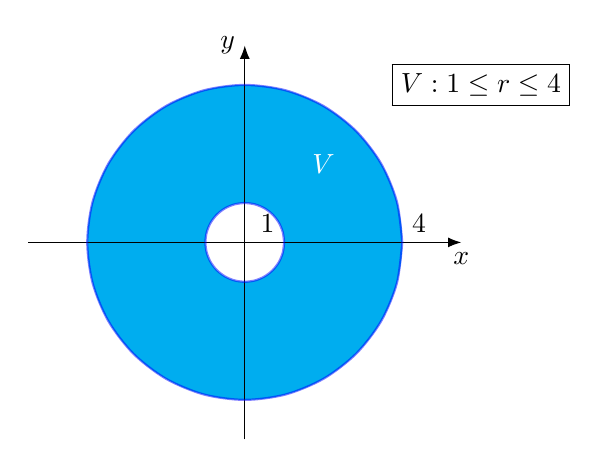
\begin{tikzpicture}[scale=0.5]
                \fill[cyan] (0,0) circle (4);
                \fill[white] (0,0) circle (1);

                \draw[-Latex] (-5.5,0) -- (5.5,0) node[below] {$x$};
                \draw[-Latex] (0,-5) -- (0,5) node[left] {$y$};

                \draw[blue,thick,opacity=0.5] plot[domain=0:360,smooth,variable=\t] ({4*cos(\t)},{4*sin(\t)});
                \draw[blue,thick,opacity=0.5] plot[domain=0:360,smooth,variable=\t] ({1*cos(\t)},{1*sin(\t)});
                
                \node at (1,0) [above left] {$1$};
                \node at (4,0) [above right] {$4$};

                \node at (2,2) {\color{white}$V$};
                \node at (6,4) {$\boxed{V:1\leq r \leq 4}$};
            \end{tikzpicture}
        \end{center}
        Dengan menggunakan koordinat silinder, didapatkan $dV=|r|\, dr\, d\theta\, dz$ dengan $|r|$ adalah jacobian dari koordinat silinder.
        \begin{flalign*}
            2\iiint_V z\, dV&=2\int_0^{2\pi}\int_1^4\int_0^2 z\, |r|\, dz\, dr\, d\theta&\\
            &=2\int_0^{2\pi}\int_1^4\left[\frac{1}{2}z^2\right]_0^2\, r\, dr\, d\theta&\\
            &=4\int_0^{2\pi}\int_1^4 r\, dr\, d\theta&\\
            &=4\int_0^{2\pi}\left[\frac{1}{2}r^2\right]_1^4\, d\theta&\\
            &=4\int_0^{2\pi}\left[\frac{1}{2}(4^2-1^2)\right]\, d\theta&\\
            &=2\int_0^{2\pi}15\, d\theta&\\
            &=2\cdot 15\cdot 2\pi=\boxed{60\pi}
        \end{flalign*}
    \end{enumerate}
\end{document}